\subsection{Can Power Sensor Readings be Used?}
\label{subsec:modelling_sensor}

Since using the built-in power sensor readings would allow SPMD to be performed on any phone in the wild,
we assess the feasibility of using the power sensors in modern smartphones for developing SPMD,
by measuring the accuracy of their the energy counter readings.

%{\bf Methodology }
%% 2. Explanation of equation generation
% Since in principle, the energy counter gives more accurate energy estimation for an equation interval than averaging all the instantaneous power readings in the interval multiplied by the interval duration,
% we use energy counter readings to generate the LHD of each model equation.
\begin{sloppy}
% The Android versions on both phones exports APIs for power sensor readings with
Android 7.0 and later provide 
interfaces to the built-in power sensor through sysfs~\cite{linuxsysfs} with
a finite sampling resolution, 1.4s on Pixel 2 and Moto Z3 and 380 ms on Pixel 4.
\comment{The power sensor readings have two formats}: instantaneous power draw 
({\small /sys/\-class/\-power\_supply/\-battery/\-current\_now}) and
energy counter ({\small /sys/\-class/\-power\_supply/\-battery/\-charge\_counter})
which reports the total energy in the previous sampling interval.
\end{sloppy}

\begin{figure}[tp]
    \centering
\if 0
\begin{subfigure}[b]{0.50\textwidth}
         \centering
         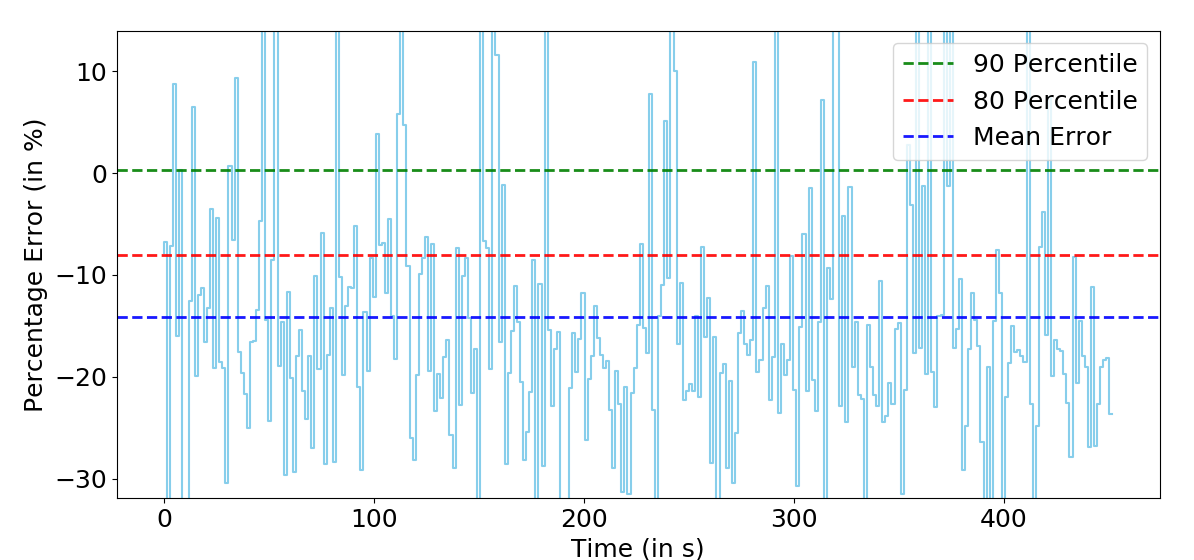
\includegraphics[width=\textwidth]{figures/sensor_error_timeline_5.png}
         \caption{Timeline on Moto Z3}
         \label{fig:sensor_error_timeline}
     \end{subfigure}
     \hfill
\fi

\begin{minipage}{0.48\columnwidth}
\begin{subfigure}[b]{\textwidth}
         \centering
         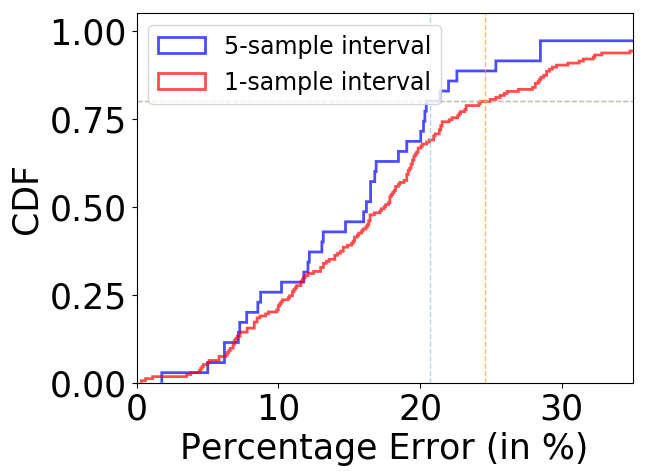
\includegraphics[width=\textwidth]{figures/sensor_error_cdf.png}
         % \caption{CDF for Moto Z3}
%         \label{fig:sensor_error_cdf_motoz3}
     \end{subfigure}
     
  \if 0
  \begin{subfigure}[b]{0.46\columnwidth}
         \centering
         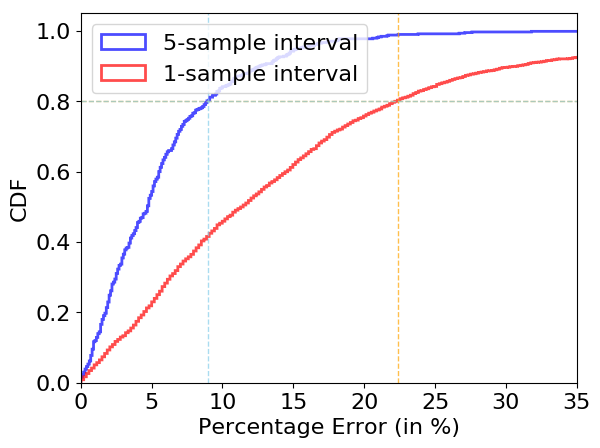
\includegraphics[width=\textwidth]{figures/sensor_error_cdf_nexus6.png}
         \caption{CDF for Nexus 6}
         \label{fig:sensor_error_cdf_nexus6}
     \end{subfigure}
  \fi
  \caption{Power sensor reading error relative to power monitor reading
        for the YouTube for Moto Z3.
        % In CDF, the orange line represents the 80 percentage for 1 sample and blue line represents for 5 sample
        }
        \label{fig:sensor_error}
        \vspace{-0.1in}
\end{minipage}
\hfill
\begin{minipage}{0.48\columnwidth}

    \centering
    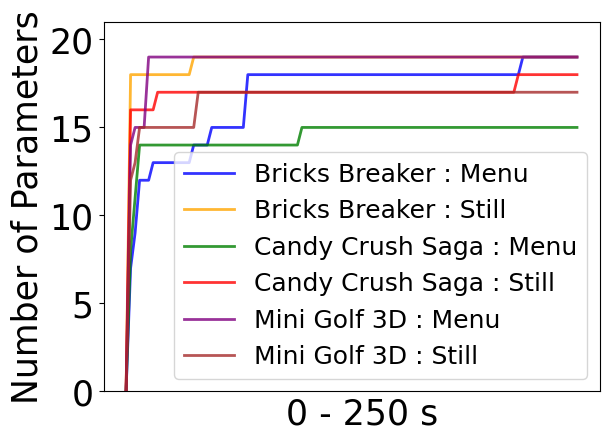
\includegraphics[width=\textwidth]{figures/004_Pixel4_cummulative_macro_parameters.png}
    \vspace{-0.1in}
    \caption{The cumulative number of unique parameters over app run duration on Pixel 4.}
    \label{fig:number_parameters_vs_duration}
    \vspace{-0.1in}
\end{minipage}
\end{figure}


 
To validate the energy counter reading accuracy comparing it with the high-fidelity 
external power monitor readings as the ground truth,
we generated a 250-second run with the YouTube app while the device is connected to the power monitor.
We chose YouTube as it is a popular app and exhibits significant power variations during its run.

%{\bf Findings}
%% 3. Explain power sensor is effects the accuracy of the equations
%Figure~\ref{fig:sensor_error} shows the timeline and the CDF for the sensor error.
\if 0
Figure~\ref{fig:sensor_error_timeline} shows the percentage error of the estimated energy
for 1-sample intervals (1.4s) based on power sensor reading over the 500s app run for Moto Z3.
We observe that \comment{for 89.7\% of the intervals the power sensor reading underestimates the energy drain compared to the power monitor reading.}
\fi

Figure~\ref{fig:sensor_error} shows the CDF for the absolute percentage error on Moto Z3
for 1-sample and for 5-sample intervals (7s). 
We plot the error for 5-sample intervals to see if averaging out over 5 samples can reduce the 
power sensor reading error.
% since if so we can set up an equation for each 5-sample interval as opposed to each 1-sample interval.
However, we see that the average error for 5-sample intervals, 15.84\%,
is only slightly better compared to 1-sample intervals of 19.01\%, and
the 80th percentile errors are 20.52\% and 24.18\% and median errors are 
16.76\% and 17.99\%., respectively.
\if 0
% , and the 80th percentile errors are 24.03\% and 21.10\%, respectively.
% Nexus 6
Figure~\ref{fig:sensor_error_cdf_nexus6} shows the CDF for the absolute percentage error
for 1-sample intervals (175 ms) and for 5-sample intervals (875 ms) for Nexus 6.
However, we see that the average error for 5-sample intervals, 7.21\%,
is lower than for 1-sample intervals of 19.06\%, and
the 80th percentile errors are 9.89\% and 26.60\%, respectively.
\comment{We observe that the sensor is about 3 times lower in Nexus 6 as compared to Moto Z3
for 1 sample interval is due to the interval of Nexus 6 being 8 times shorter than Moto Z3.
Suggesting that the low sampling rate of the sensor is the cause of the error.}
\fi
Such high error suggests that the built-in power sensor readings available on today's Android phones 
are not suitable for self power model derivation. 
Thus we conduct our SPMD verification study by using the external Monsoon power monitor to generate the 
power draw ground truth. 

\if 0
{\bf Reason }
%% 5. Reasons for the inaccuracies in power sensor
The high inaccuracy of the power sensor could be attributed to mainly 2 reasons.
\begin{itemize}
    \item {\bf Noise: } The power management circuit and it's location in the device is susceptible to noise due to the electronic circuitry involved in it.
    It can be argued that, the noise can be reduced by taking a longer interval which might average out the effect of noise, but from our finding we find that this approach is not effective.
    
    \item {\bf Low Sampling rate: } The power sensor generate a new value every 1.4 seconds interval in moto Z3.
    This greatly inhabits use of the power sensor to gather instantaneous current. 
 \end{itemize}
\fi


% The Monsoon power monitor has a sampling rate of 5 KHz  and has been widely used as the ground truth in smartphone power modeling and energy drain studies. 
